\section{Theoretical background}
\subsection{Time Series data}
Typically, a time series data is the repeated measurement of parameters over time together with the times at which the measurements were made~\cite{time_series_databases}. Time series often consist of measurements made at regular intervals, but the regularity of time intervals between measurements is not a requirement. As an example, the temperature measurements for the last week with the timestamp for each measurement is a time series temperature data. The time series data is most commonly used for analytical purposes, including machine learning for predictive analysis. A single value of such data could be both a direct measurement from a device or some calculated value, and as long as it has some sort of timestamp to it, the series of such values could be considered a time series.

\subsection{IoT data and Edge computing}
Nowadays the term "time-series data" is well-known due to the recent growth in popularity of the Internet of Things, or IoT, devices, and solutions, since an IoT device is often used to collect some measure in a form of time-series data. Often this data is transferred to a server for analytical and statistical purposes. However, in a large and complex monitoring system, such as an industrial IoT, the amount of data being generated causes various problems for transferring and analyzing this data. A popular way of extending the capabilities of IoT system is to introduce some form of intermediate devices called "edge" devices~\cite{ind_iot_edge}. The traditional architecture of organizing a complicated IoT system is shown in Figure~\ref{fig1}.

\begin{figure}[htb]
\centering
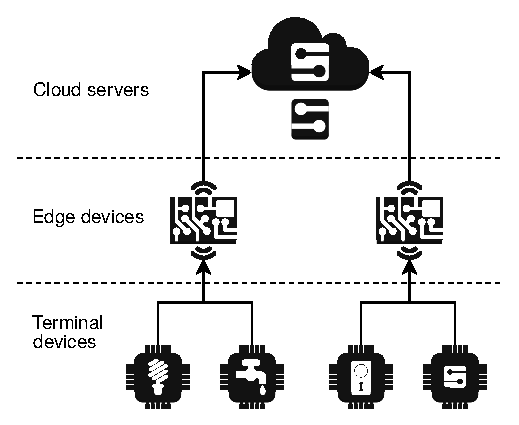
\includegraphics{figures/iot-hierarchy.drawio.eps}
\caption{An architecture of a complicated IoT system.} \label{fig1}
\end{figure}

This architecture provides flexibility in terms of data collection.
In case of problems with the network connection between the endpoint device and the cloud, data can be buffered in the edge device and then re-sent to the server when the connection is established. Therefore, an edge device should have the possibility to accumulate the data from the IoT devices for those periods of the network outage. However, often an edge device is not capable to run a proper database management system apart from other applications. So there has to be a way to embed the storing of time-series data to an existing application. From this point an assumption will be made that the application is written in a Go programming language because this language maintains the balance between complexity, being easier to use than C/C++, and resource inefficiency, being less demanding than Python.

\subsection{In-app data storage}
Traditionally, either some form of in-memory data structures or embedded databases are used to store data within the application. However, if data is critical and it is important not to lose it in case of a power outage, in-memory storage doesn't fit. An embedded database, or other forms of persistent data storage that is used within the application, reduces the access speed compared to any in-memory storage system. This article describes an LSM-based storage system. This type of system is providing the best of both worlds - persistent data storage with fast data access.